\section{Data}\label{appx:data}

\subsection{Phoneme grouping in TIMIT dataset}\label{appx:timit-phonemes}
Phonemes are fundamental units of speech, detailing the pronunciation of a word.
The TIMIT dataset provides phoneme annotations in addition to text annotations, with phoneme durations in the 10-400 millisecond range. 
\cite{astolfi_duration_2015}

The Phonemes in the TIMIT dataset were grouped as described by the authors.
\cite{garofolo_john_s_timit_1993}
\Cref{tab:timit-phonemes} shows the groupings used in this work.
We keep the closure intervals of stops, denoted by a \texttt{*cl}, separated from the corresponding stop release, instead of keeping the groupings. 
The start and stop token, \texttt{h\#} was omitted in phoneme mapping to latent spaces.

\subsection{Phoneme lengths in the TIMIT dataset}\label{appx:timit-phoneme-duration}
\Cref{fig:timit-phoneme-duration} shows the length of phonemes pronouced in the TIMIT validation set. 




\begin{table}[htb]
    \centering
    \begin{tabular}{r|p{8cm}}
        Group & Phonemes \\
        \hline
        Vowels & \texttt{iy, ih, eh, ey, ae, aa, aw, ay, ah, ao, oy, ow, uh, uw, ux, er, ax, ix, axr, ax-h} \\
        Stops & \texttt{b, d, g, p, t, k, dx, q} \\
        Closures & \texttt{bcl, dcl, gcl, pcl, tck, kcl, tcl} \\
        Affricates & \texttt{jh, ch} \\
        Fricatives & \texttt{s, sh, z, zh, f, th, v, dh} \\
        Nasals & \texttt{m, n, ng, em, en, eng, nx} \\
        Semivowels and Glides & \texttt{l, r, w, y, hh, hv, el} \\
        Others & \texttt{pau, epi, h\#, 1, 2} \\ 
    \end{tabular}
    \caption{TIMIT phoneme groupings}
    \label{tab:timit-phonemes}
\end{table}


\begin{figure}[t!]
    \centering
    \hfill
    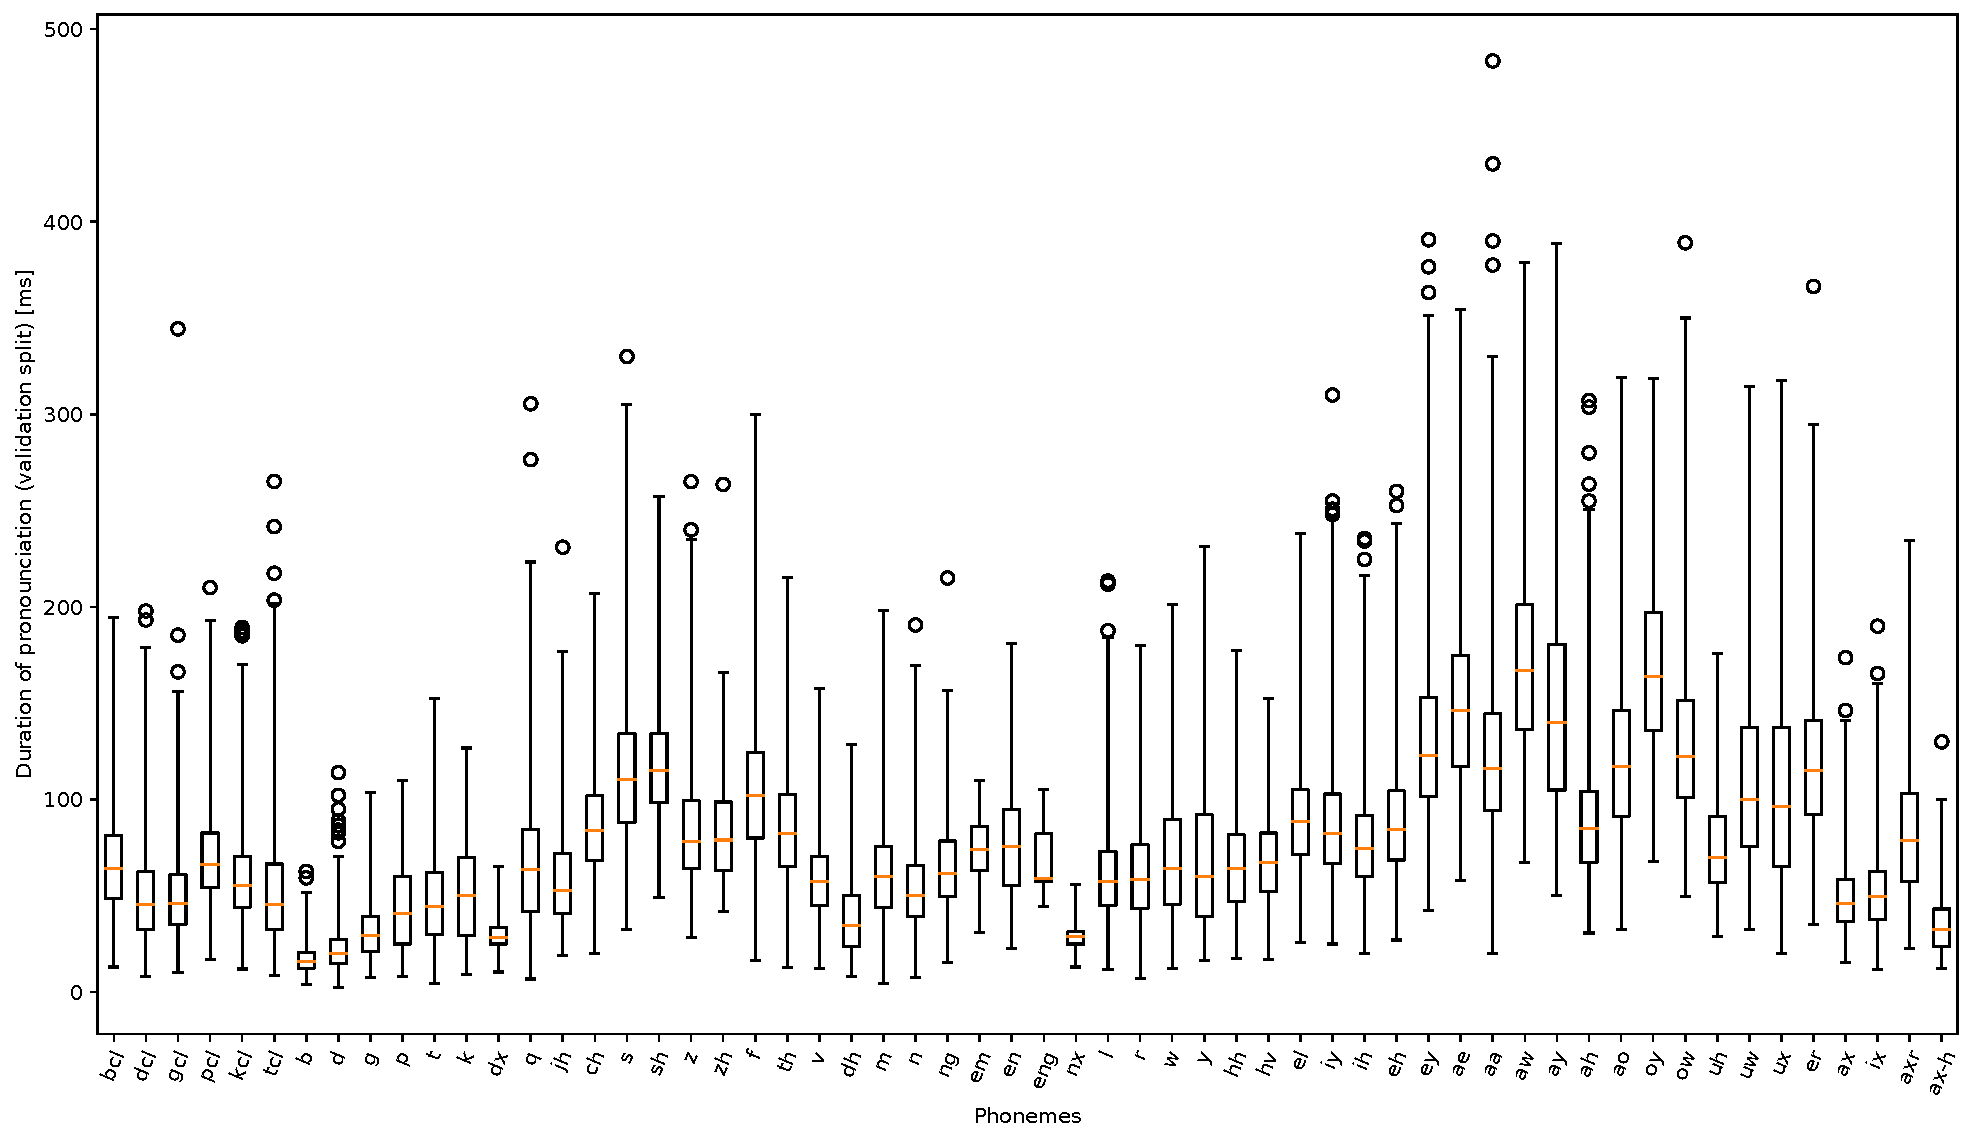
\includegraphics[width=\textwidth]{gfx/TIMIT_validation_set_phoneme_duration_boxplot_speaker_id_None.pdf}
    \caption{Boxplot of the duration of the pronunciation of phonemes in the TIMIT validation set.}
    \label{fig:timit-phoneme-duration}
\end{figure}
